\subsection{INFINITE SERIES AND INFINITE PRODUCTS OF REAL NUMBERS}

A series of finite real numbers is simply said to be convergent if it is convergent in R.

DEFINITION 1. A series of finite real numbers is said to be absolutely convergent if the series of absolute values of its terms is convergent.

PROPOSITION 4. A series of finite real numbers is commutatively convergent if and only if it is absolutely convergent.

This follows from Chapter III, § 5, no. 7, Proposition 9 and from Theorem 3 of no. 2.

In other words, if \((u_{n})\) is a sequence of finite real numbers, it comes to the same thing to say that the series whose general term is \(u_{n}\) is commutatively convergent, or that it is absolutely convergent, or that the sequence \((u_{n})\)

is summable in \(\mathbf{R}\) . All the properties of summable families proved in Chapter III, § 5 therefore apply to absolutely convergent series. In particular, if the series whose general term is \(u_{n}\) is absolutely convergent, then the sum \(\sum_{n\in\mathbf{H}} u_{n}\) exists for all subsets \(\mathbf{H}\) of \(\mathbf{N}\) ; and, if \((\mathbf{H}_{p})\) is a partition of \(\mathbf{N}\) , we have

\[
\sum_ {n = 0} ^ {\infty} u _ {n} = \sum_ {p} \left(\sum_ {n \in \mathrm{H} _ {p}} u _ {n}\right)
\]

(associativity of absolutely convergent series).

As we have already remarked in Chapter III, § 5, a series of real numbers can be convergent without being commutatively convergent, that is, without being absolutely convergent.

Example. Alternating series. A series defined by a sequence \((u_n)\) of finite real numbers is called alternating if \(u_n = (-1)^n v_n\) , where \(v_n \geqslant 0\) for all \(n\) . Let us show that a sufficient condition for the convergence of such a series is that the sequence \((v_n)\) decreases and has \(0\) as its limit. For if \(s_n\) denotes

\[
\sum_ {p = 0} ^ {n} u _ {p},
\]

the hypothesis that \((v_{n})\) is decreasing implies that

\[
s _ {2 n + 1} \leqslant s _ {2 n + 3} \leqslant s _ {2 n + 2} \leqslant s _ {2 n}
\]

for all \(n \geqslant 0\) . The sequence \((s_{2n})\) {[}resp. \((s_{2n+1})\) {]} is decreasing and bounded below (resp. increasing and bounded above) and therefore has a finite limit a (resp. b), and \(b \leqslant a\) ; since

\[
a - b = \lim _ {n \rightarrow \infty} (s _ {2 n} - s _ {2 n + 1}) = \lim _ {n \rightarrow \infty} v _ {2 n + 1} = 0,
\]

the assertion is proved.

If we take for example \(v_{n}=1/n\) , the conditions above are satisfied, and therefore the series whose general term is \((-1)^{n}/n\) (the ``alternating harmonic series'') is convergent. We have seen in no. 1 that the series whose general term is 1/n (the ``harmonic series'') is not convergent, and thus the alternating harmonic series is not absolutely convergent.

We recall (Chapter III, § 5, no. 6, Proposition 7) that, if \((u_n)\) and \((v_n)\) are two convergent series of finite real numbers, then the series \((u_n + v_n)\) is convergent, and

\[
\sum_ {n = 0} ^ {\infty} \left(u _ {n} + v _ {n}\right) = \sum_ {n = 0} ^ {\infty} u _ {n} + \sum_ {n = 0} ^ {\infty} v _ {n};
\]

also, if the series \((u_{n})\) is convergent then the series \((au_{n})\) is convergent for all finite real numbers \(a\) , and \(\sum_{n=0}^{\infty} au_{n} = a\) . \(\sum_{n=0}^{\infty} u_{n}\) .

Finally, if the series \((u_n)\) and \((v_n)\) are convergent, and if \(u_n \leqslant v_n\) for all \(n\) , we have \(\sum_{n=0}^{\infty} u_n \leqslant \sum_{n=0}^{\infty} v_n\) by the principle of extension of inequalities (§ 5, no. 2, Theorem 1).

It should be noted that, if we suppose the series \((v_{n})\) to be convergent but not absolutely convergent, and if \(|u_{n}| \leqslant |v_{n}|\) for each n, we can by no means infer that the series \((u_{n})\) is convergent, as is seen by taking \(u_{n} = |v_{n}|\) .

An infinite product of finite non-zero real numbers is said simply to be convergent if it is convergent in \(\mathbf{R}^*\) ; its value is then a finite non-zero real number.

DEFINITION 2. An infinite product whose general factor is \(1 + u_{n}\) is said to be absolutely convergent if the product whose general factor is \(1 + |u_{n}|\) is convergent.

PROPOSITION 5. An infinite product of finite real numbers is commutatively convergent if and only if it is absolutely convergent.

This follows from Chapter III, § 5, no. 7, Proposition 9, and from Theorem 4 above.

Moreover, the product whose general factor is \(1 + u_{n}\) is absolutely convergent if and only if the series whose general term is \(u_{n}\) is absolutely convergent.

A product of non-zero real numbers can be convergent without being commutatively convergent, i.e.~without being absolutely convergent.

Example. If we take \(u_{2n-1} = -\frac{1}{n}\) and \(u_{2n} = \frac{1}{n}\) for \(n \geqslant 2\) , the product \((1 + u_n)\) is not absolutely convergent, since the series \((u_n)\) is not absolutely convergent; but since

\[
\begin{array}{l} \prod_ {p = 3} ^ {n} (1 + u _ {p}) = \prod_ {p = 2} ^ {n} \left(1 - \frac {1}{p ^ {2}}\right), \\ \text { and } \quad \prod_ {p = 3} ^ {2 n + 1} (1 + u _ {p}) = \left(1 - \frac {1}{n + 1}\right) \prod_ {p = 2} ^ {n} \left(1 - \frac {1}{p ^ {2}}\right), \end{array}
\]

it follows from Theorem 4 that the product is convergent and that its value is

\[
\prod_ {n = 2} ^ {\infty} \left(1 - \frac {1}{n ^ {2}}\right).
\]

\pandocbounded{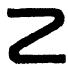
\includegraphics[keepaspectratio]{images/part003_4cdcc444.jpg}}

Moreover, it should be observed that the convergence of the series whose general term is \(u_{n}\) is neither necessary nor sufficient for the convergence of the product whose general factor is \(1 + u_{n}\) (see Exercises 21 and 22).

